
\documentclass{beamer}
\usepackage[export]{adjustbox}% http://ctan.org/pkg/adjustbox
\setbeamersize{text margin left=1cm,text margin right=1cm}
\title{Visualization of Guam Coconut Rhinoceros Beetle Trap Data\\Port Authority (PA) Traps}
%\title{' + title + ''}'
%\titlehead{Guam Coconut Rhinoceros Project Technical Report\\DRAFT: Work in progress}
%\title{Visualization of Pan Trap Data at the University of Guam Yigo Agricultural Experiment Station}
%\title{Visualization of Guam Coconut Rhinoceros Beetle Trap Data\\Port Authority (PA) Traps}

\author{Aubrey Moore}

\begin{document}
\frame{\titlepage}

\begin{frame}{Notes}
\begin{itemize}
    \item Best viewed in with a PDF reader in presentation mode.
    \item This document was generated by an IPython Notebook.
    \item Data required:
    \begin{itemize}
        \item a CSV table containing 3 fields: trap identifier and lat/long coordinates in decimal degrees
        \item a CSV table containing 4 fields: trap identifier, dates for start and end of trapping period, 
and number of beetles trapped during the trapping period
        \item a CSV table containing 2 fields: lat/long coordinates in decimal degrees defining a mask for the region of interest
    \end{itemize}
\end{itemize}
\end{frame}

\begin{frame}{Mean beetles per trap-day for 90 day period ending\\ \textbf{01 Jul 2015}}
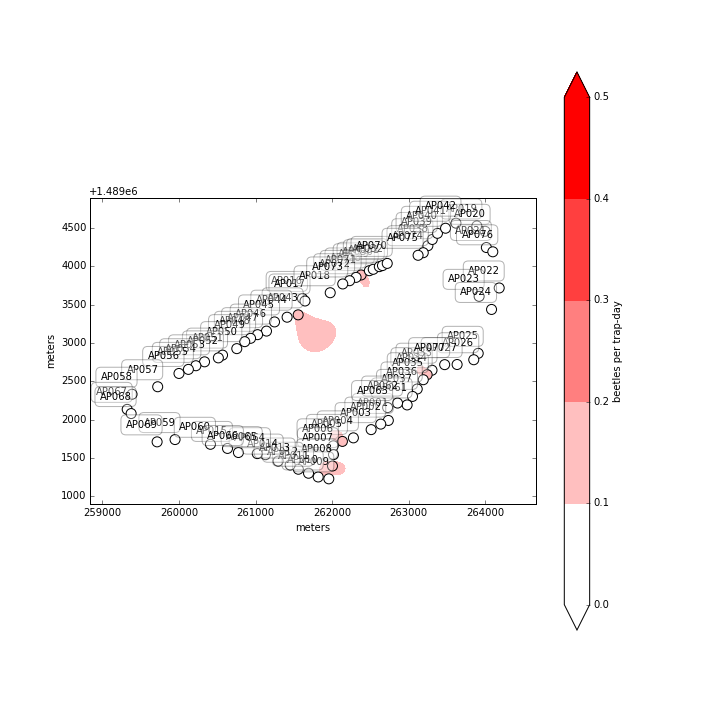
\includegraphics[width=0.6\linewidth,valign=c]{2015-07-01.png}
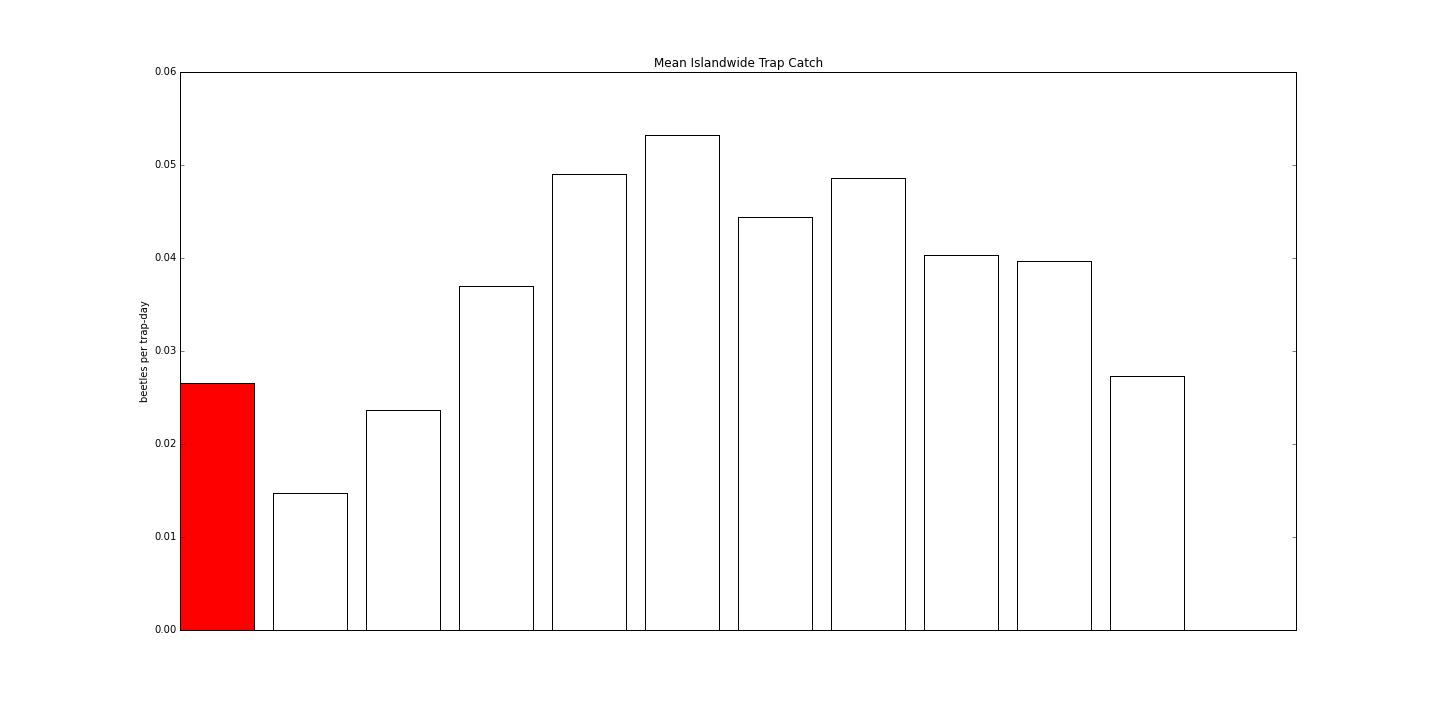
\includegraphics[width=0.4\linewidth,valign=c]{bars2015-07-01.png}
\end{frame}
\begin{frame}{Mean beetles per trap-day for 90 day period ending\\ \textbf{01 Aug 2015}}
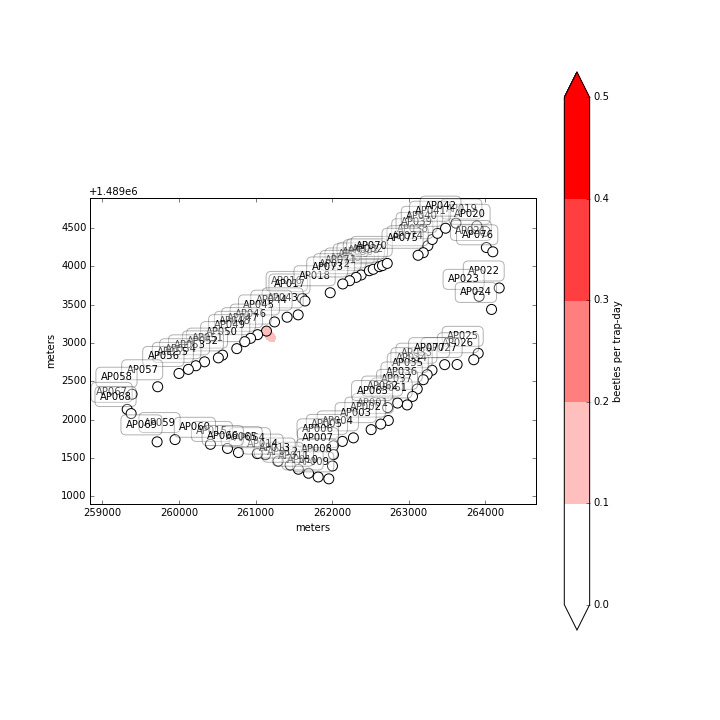
\includegraphics[width=0.6\linewidth,valign=c]{2015-08-01.png}
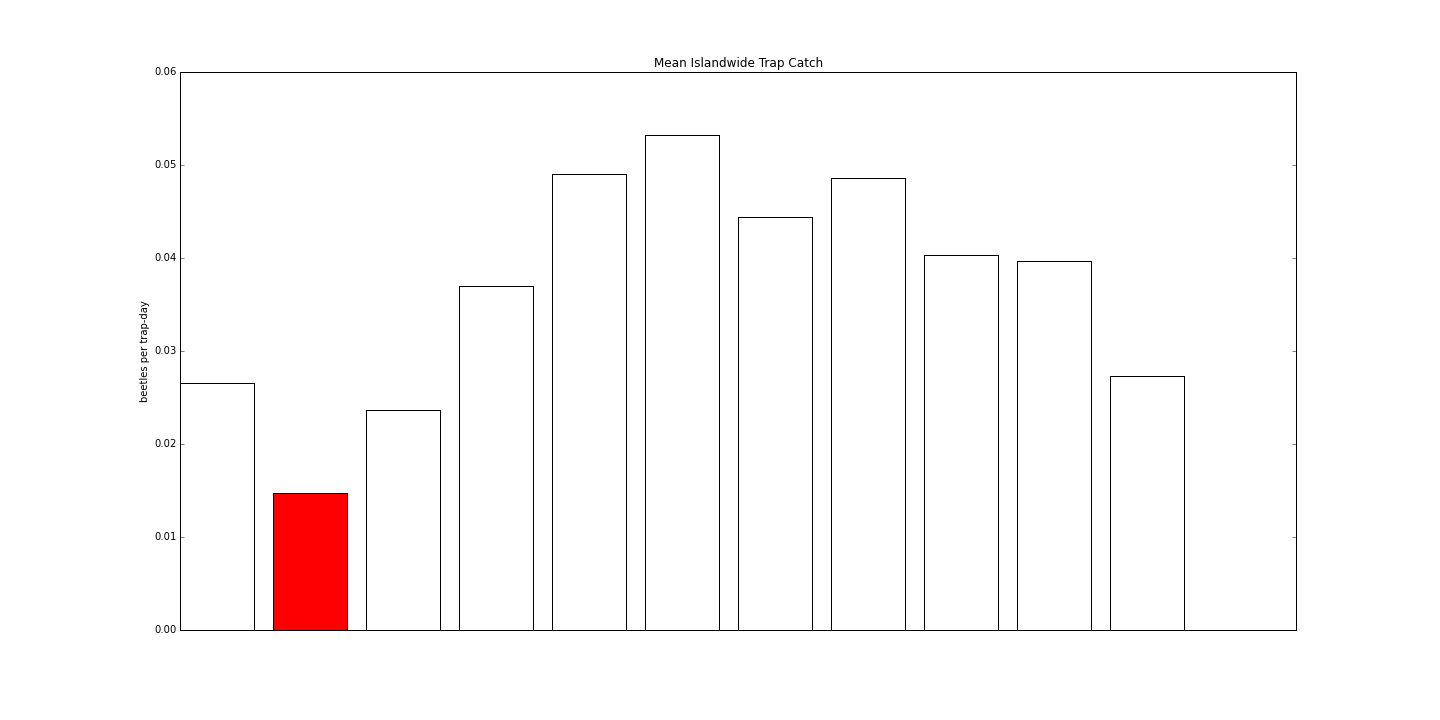
\includegraphics[width=0.4\linewidth,valign=c]{bars2015-08-01.png}
\end{frame}
\begin{frame}{Mean beetles per trap-day for 90 day period ending\\ \textbf{01 Sep 2015}}
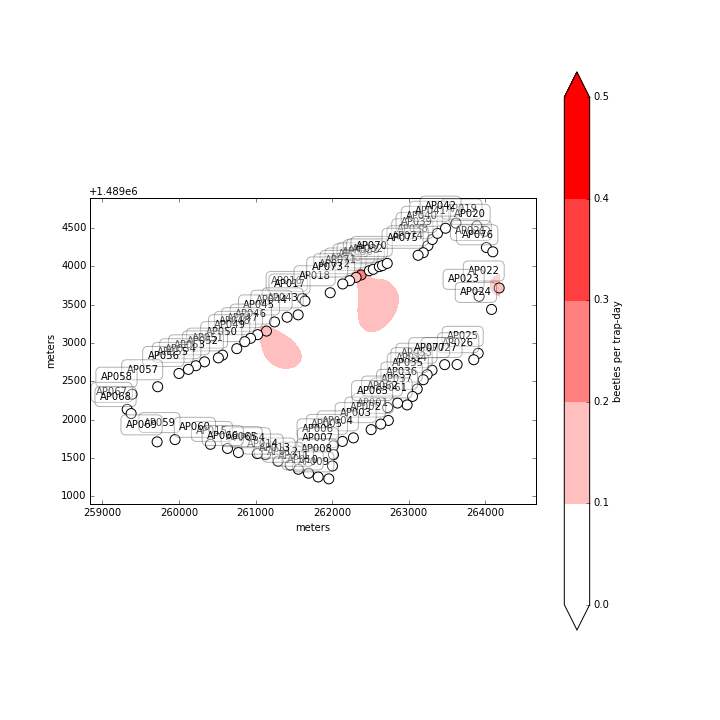
\includegraphics[width=0.6\linewidth,valign=c]{2015-09-01.png}
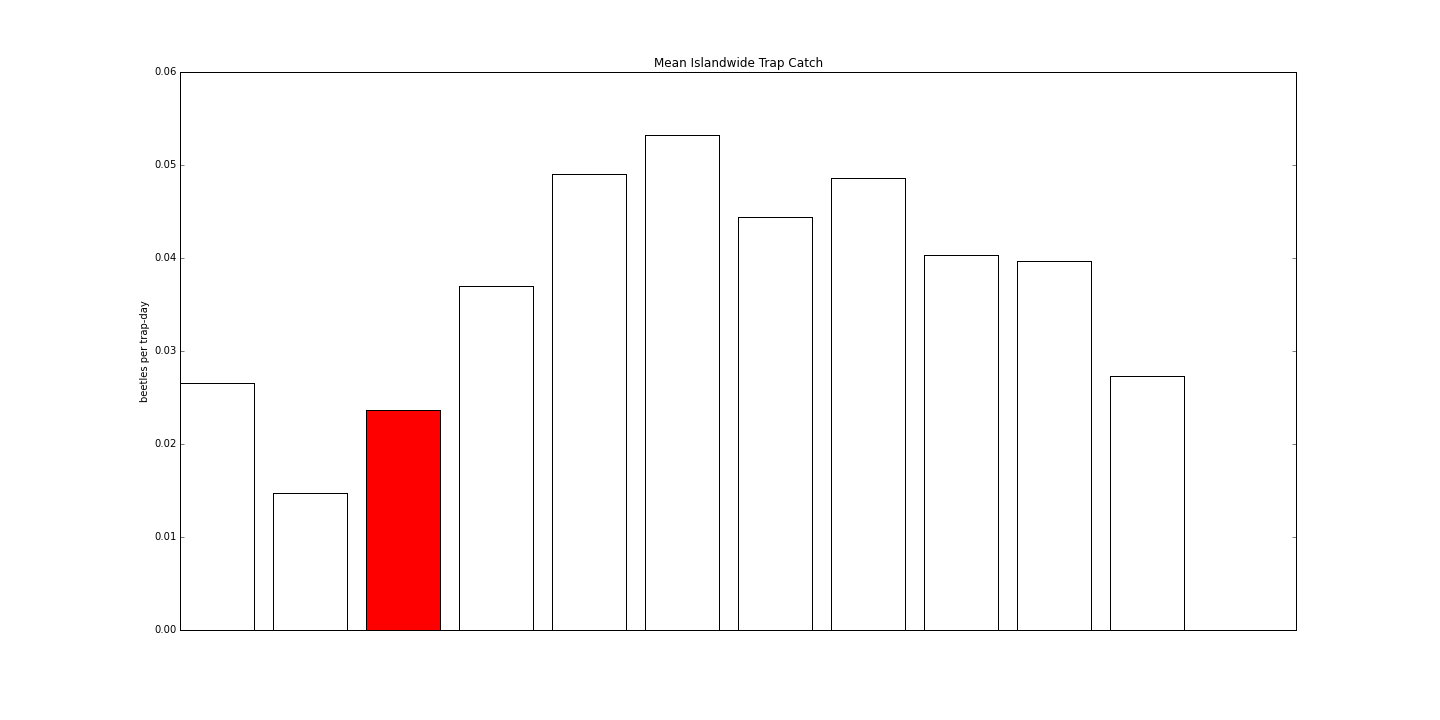
\includegraphics[width=0.4\linewidth,valign=c]{bars2015-09-01.png}
\end{frame}
\begin{frame}{Mean beetles per trap-day for 90 day period ending\\ \textbf{01 Oct 2015}}
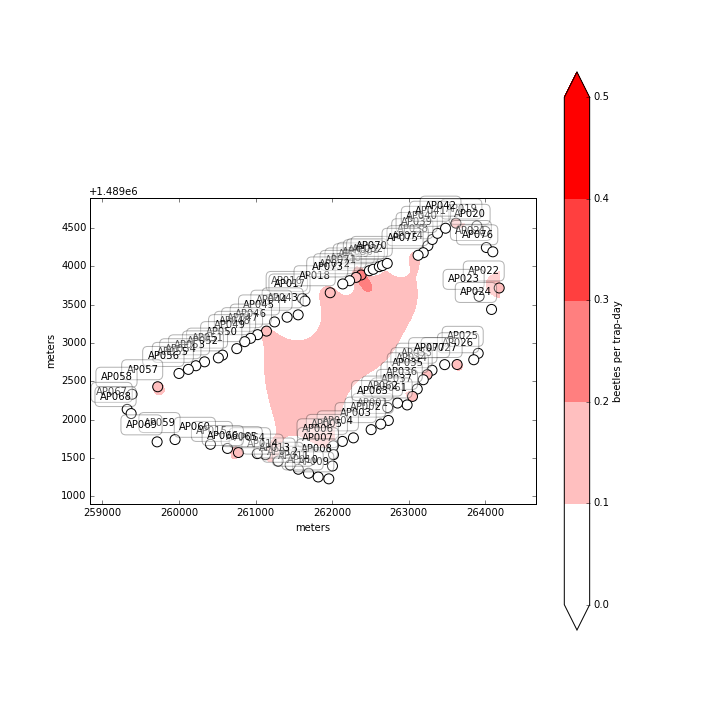
\includegraphics[width=0.6\linewidth,valign=c]{2015-10-01.png}
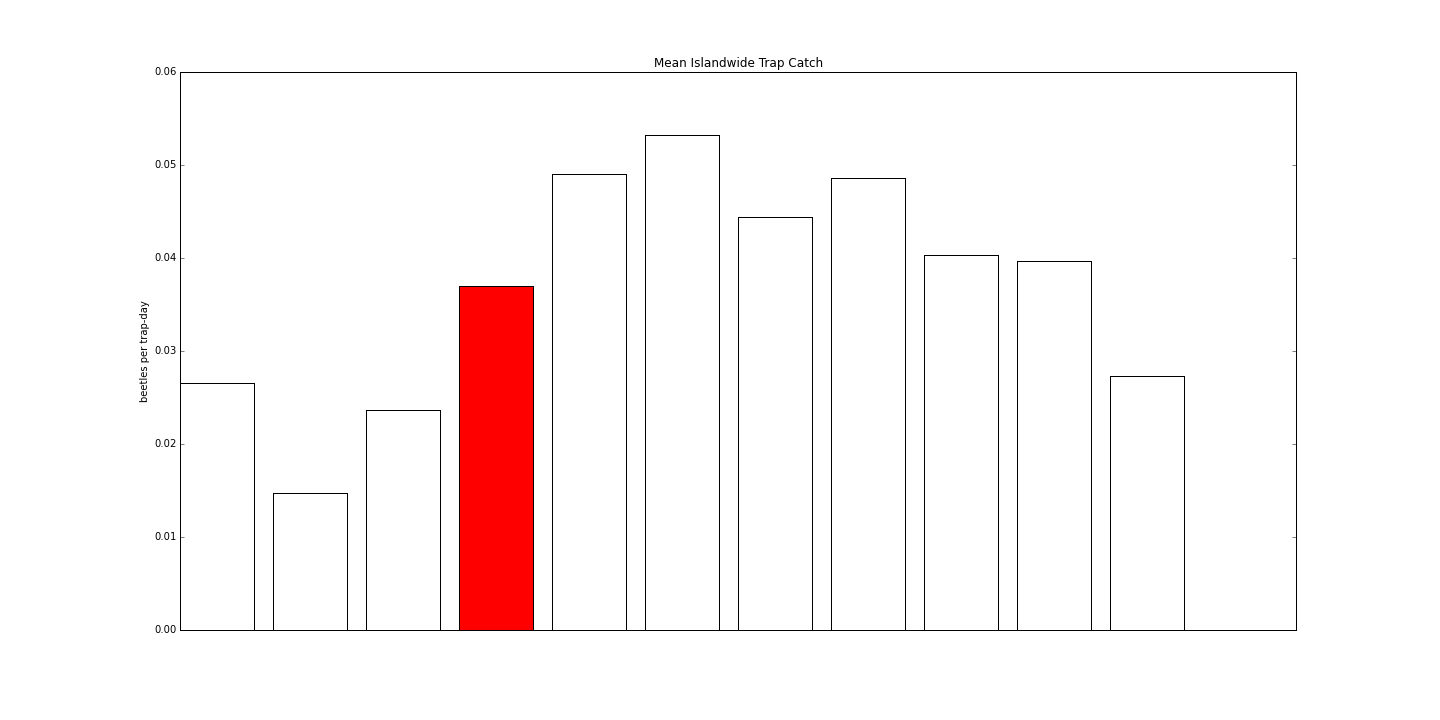
\includegraphics[width=0.4\linewidth,valign=c]{bars2015-10-01.png}
\end{frame}
\begin{frame}{Mean beetles per trap-day for 90 day period ending\\ \textbf{01 Nov 2015}}
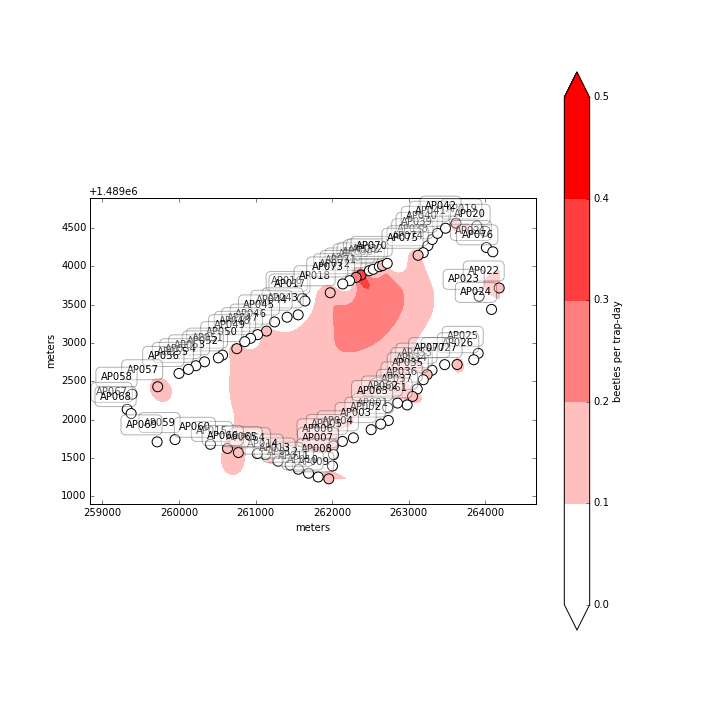
\includegraphics[width=0.6\linewidth,valign=c]{2015-11-01.png}
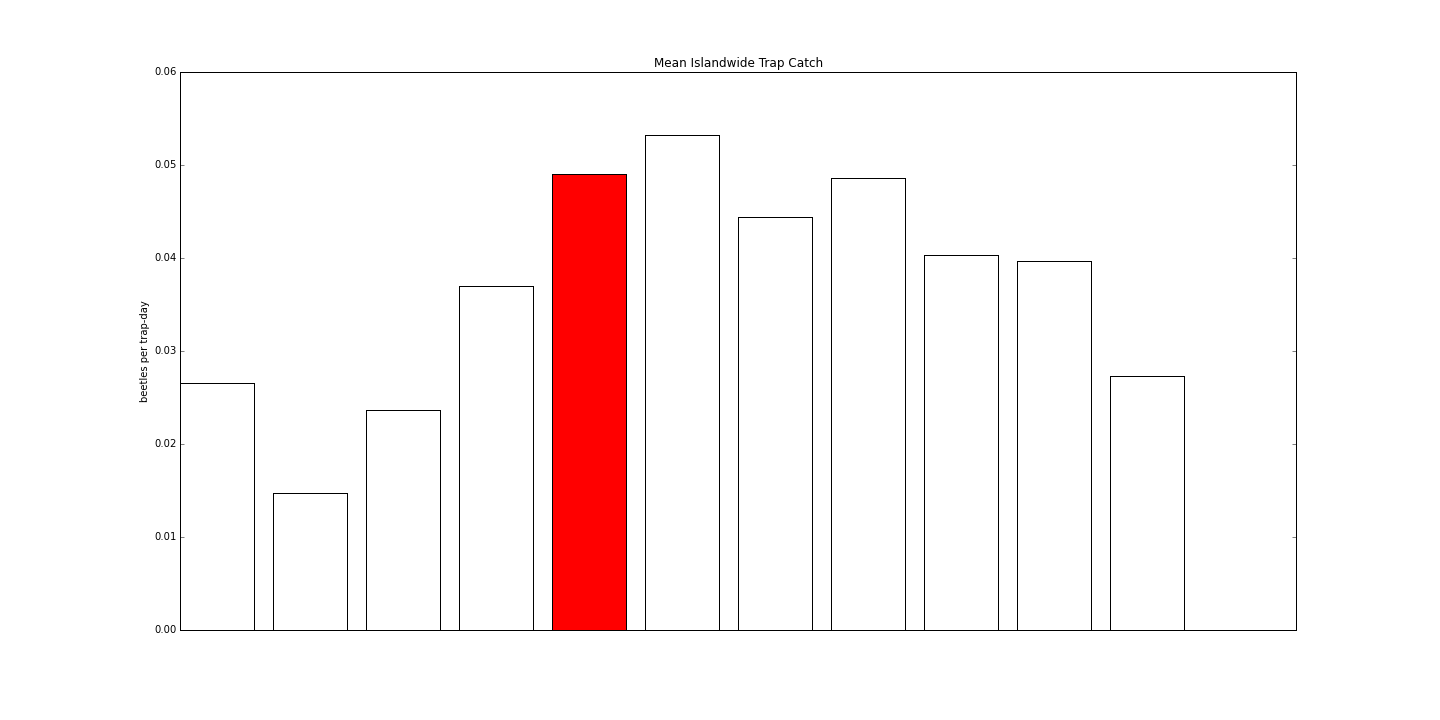
\includegraphics[width=0.4\linewidth,valign=c]{bars2015-11-01.png}
\end{frame}
\begin{frame}{Mean beetles per trap-day for 90 day period ending\\ \textbf{01 Dec 2015}}
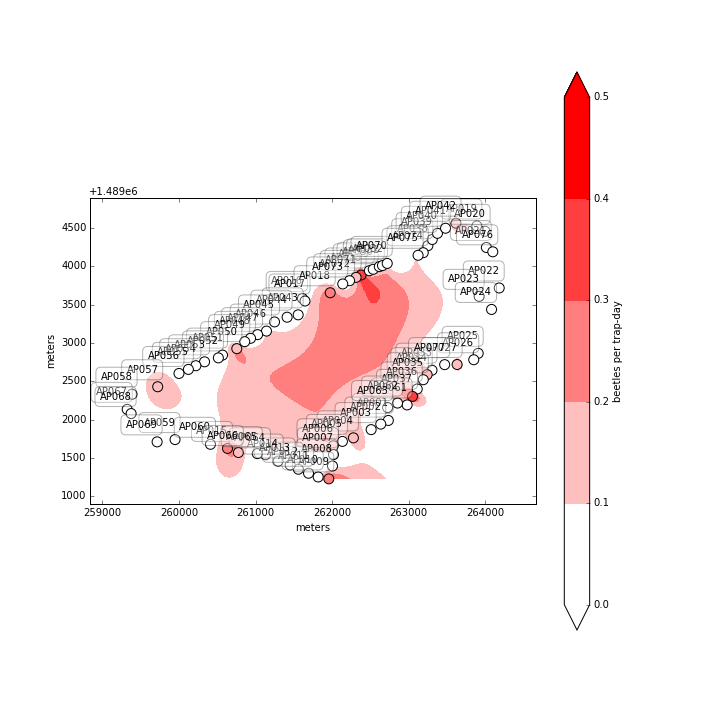
\includegraphics[width=0.6\linewidth,valign=c]{2015-12-01.png}
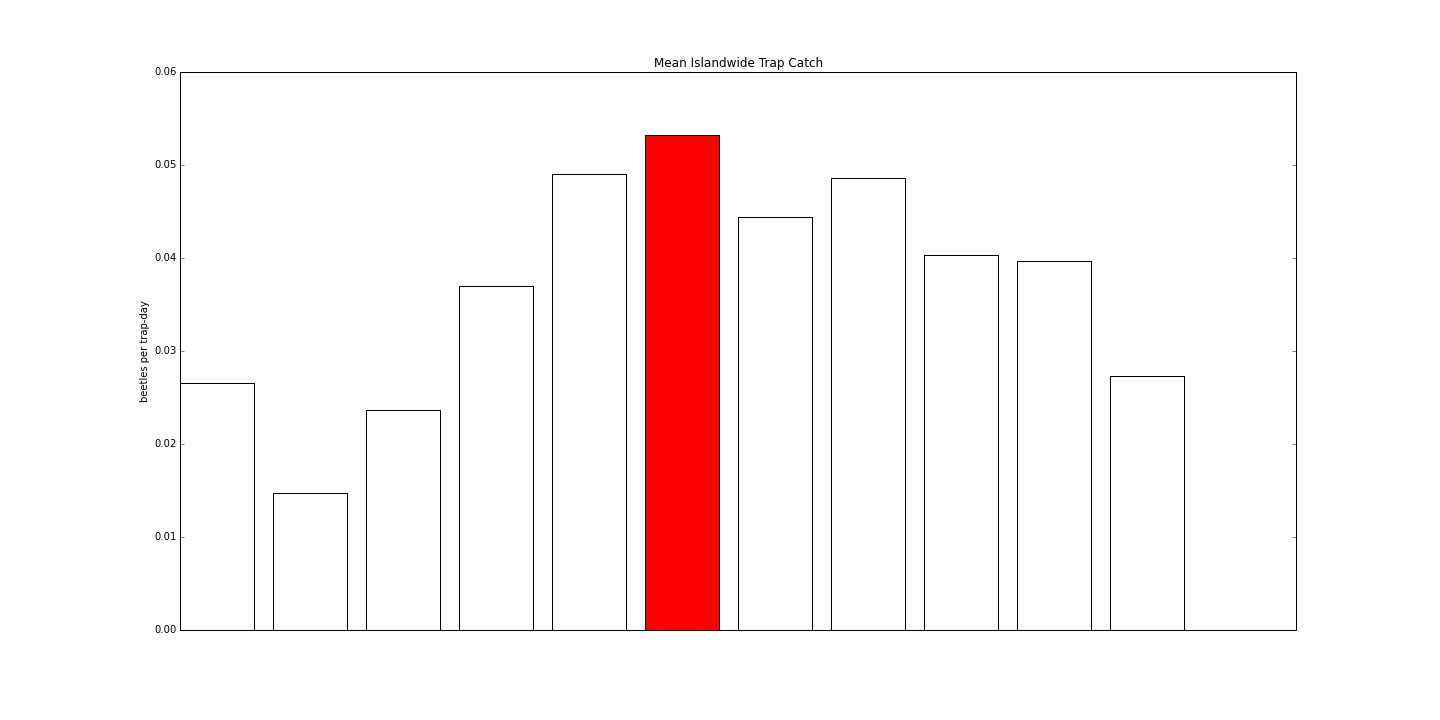
\includegraphics[width=0.4\linewidth,valign=c]{bars2015-12-01.png}
\end{frame}
\begin{frame}{Mean beetles per trap-day for 90 day period ending\\ \textbf{01 Jan 2016}}
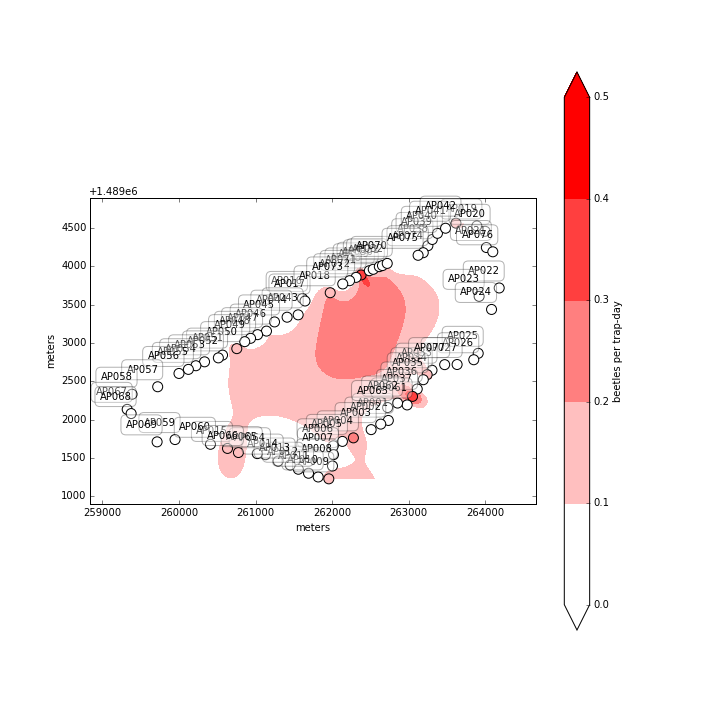
\includegraphics[width=0.6\linewidth,valign=c]{2016-01-01.png}
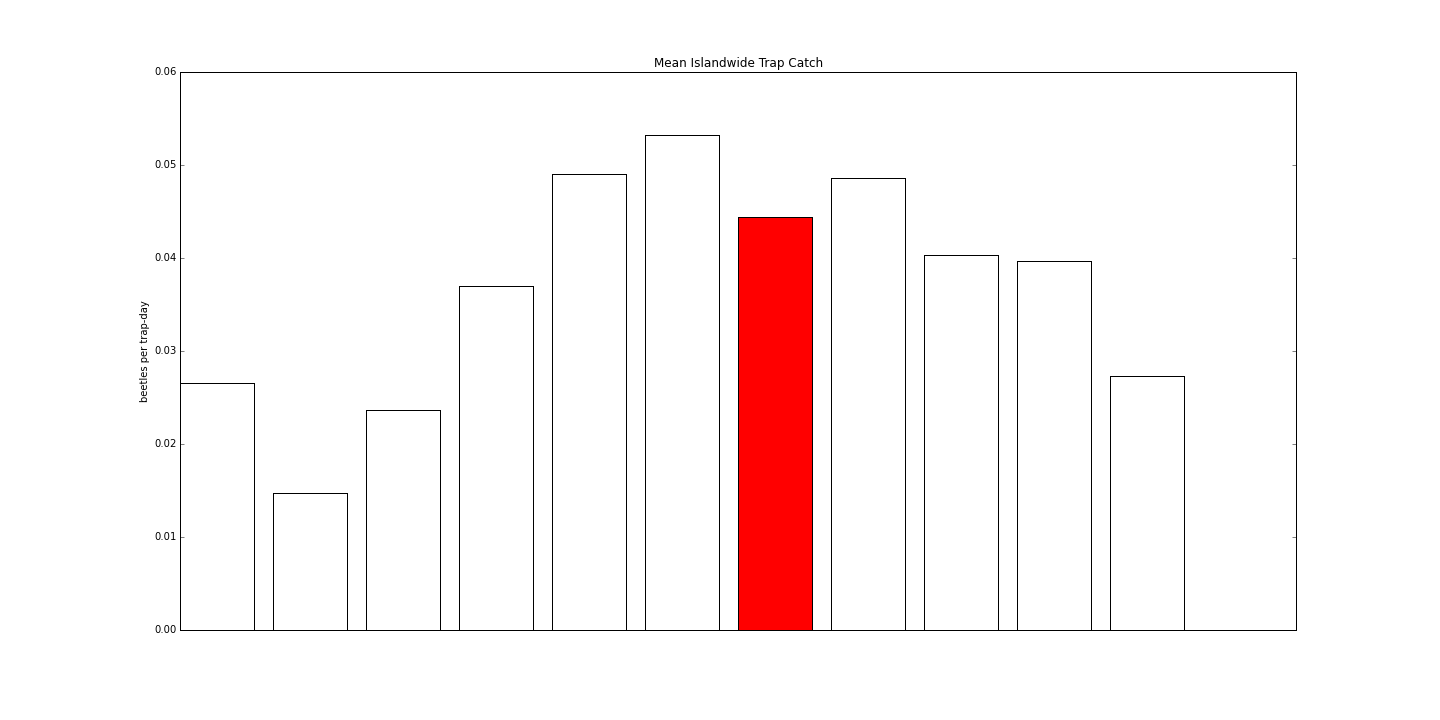
\includegraphics[width=0.4\linewidth,valign=c]{bars2016-01-01.png}
\end{frame}
\begin{frame}{Mean beetles per trap-day for 90 day period ending\\ \textbf{01 Feb 2016}}
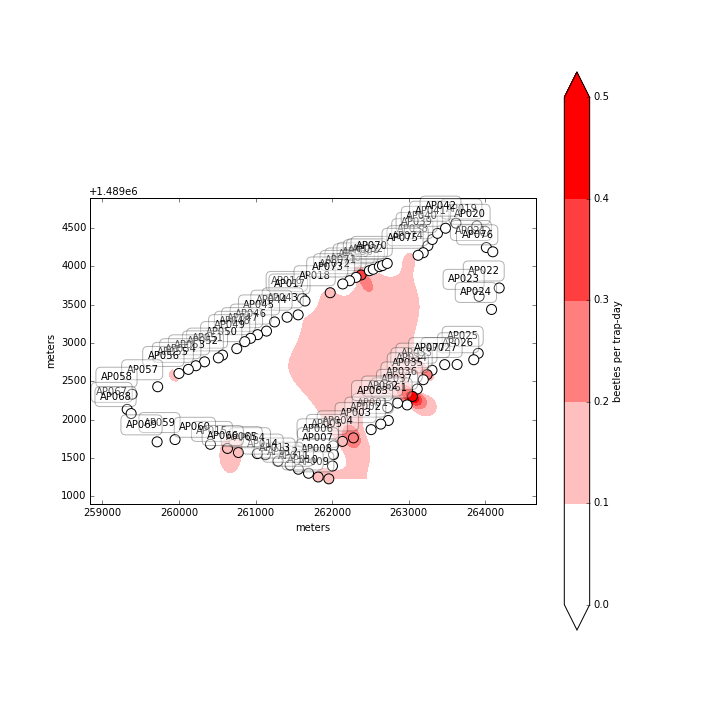
\includegraphics[width=0.6\linewidth,valign=c]{2016-02-01.png}
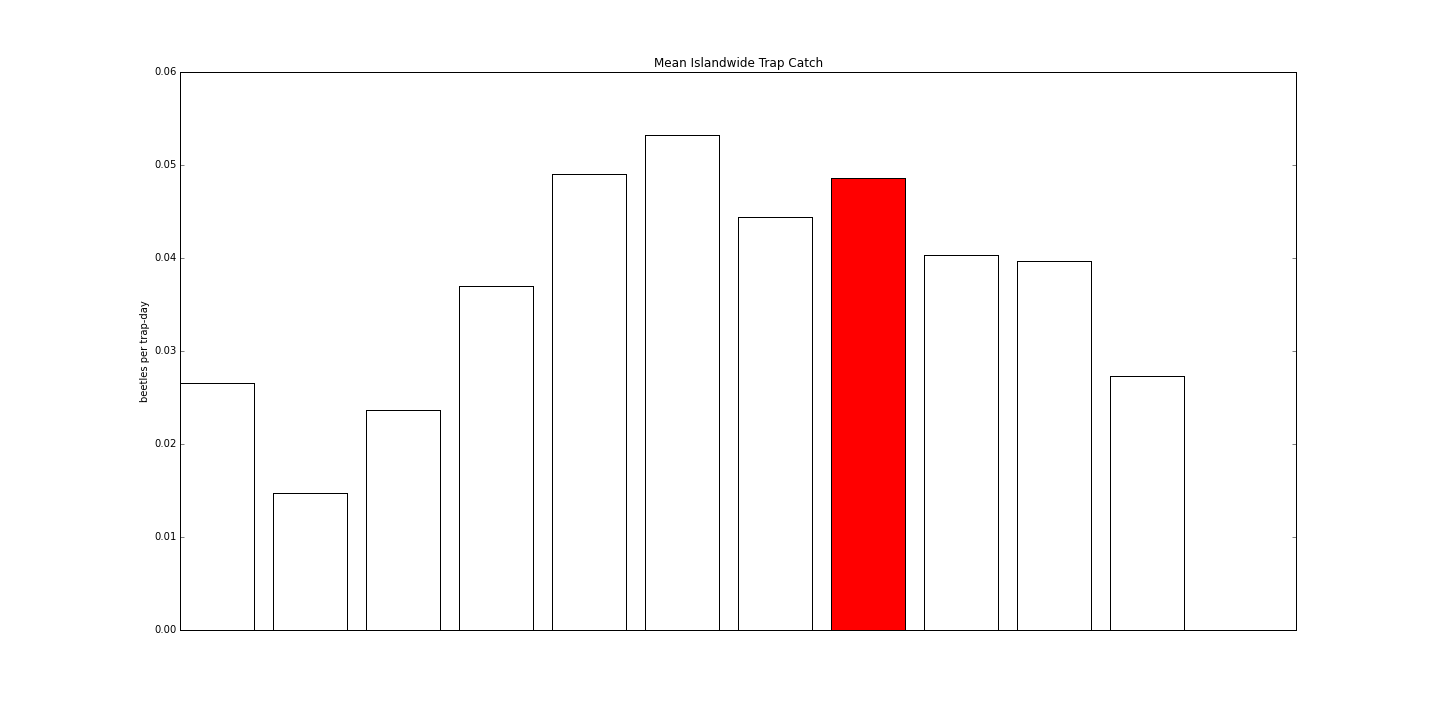
\includegraphics[width=0.4\linewidth,valign=c]{bars2016-02-01.png}
\end{frame}
\begin{frame}{Mean beetles per trap-day for 90 day period ending\\ \textbf{01 Mar 2016}}
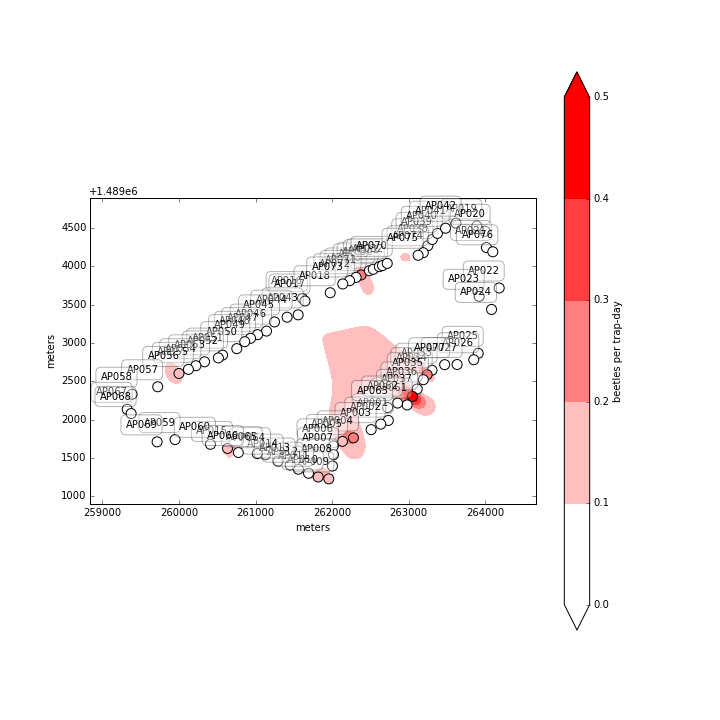
\includegraphics[width=0.6\linewidth,valign=c]{2016-03-01.png}
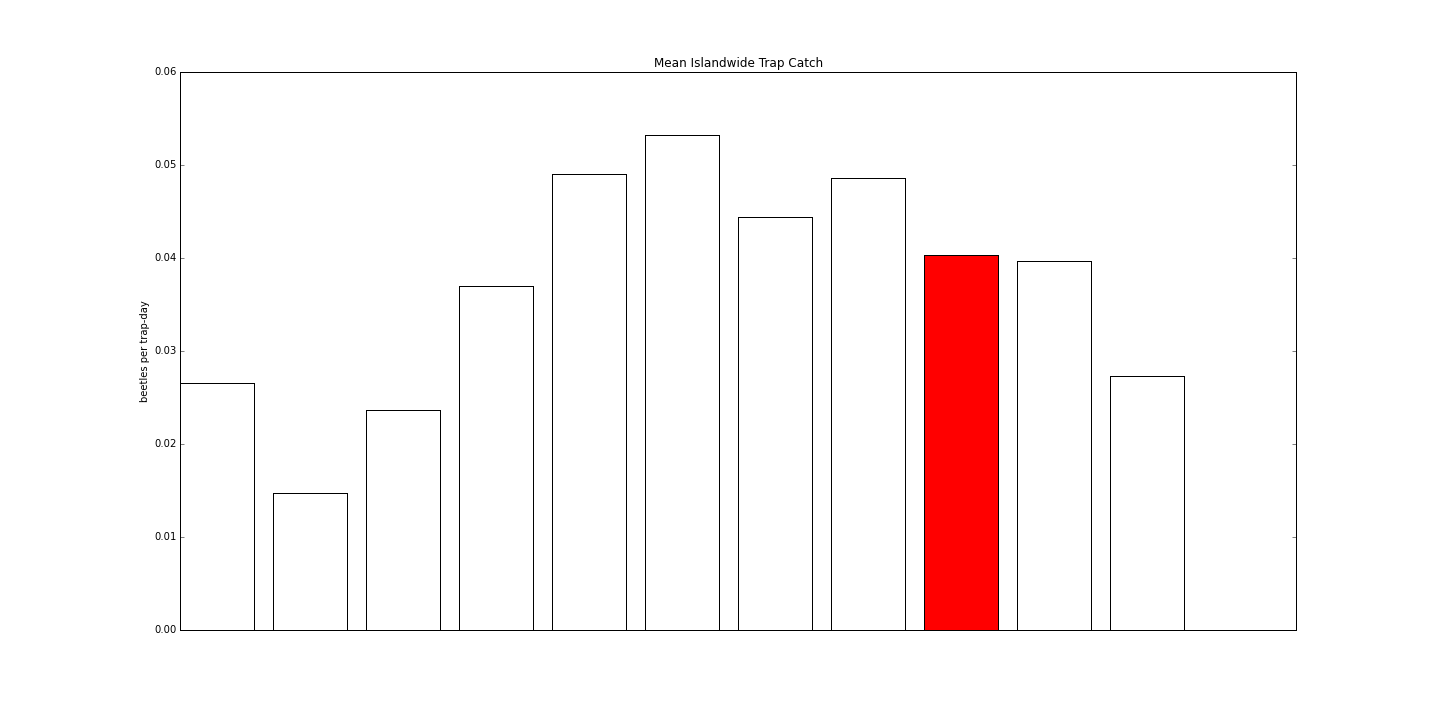
\includegraphics[width=0.4\linewidth,valign=c]{bars2016-03-01.png}
\end{frame}
\begin{frame}{Mean beetles per trap-day for 90 day period ending\\ \textbf{01 Apr 2016}}
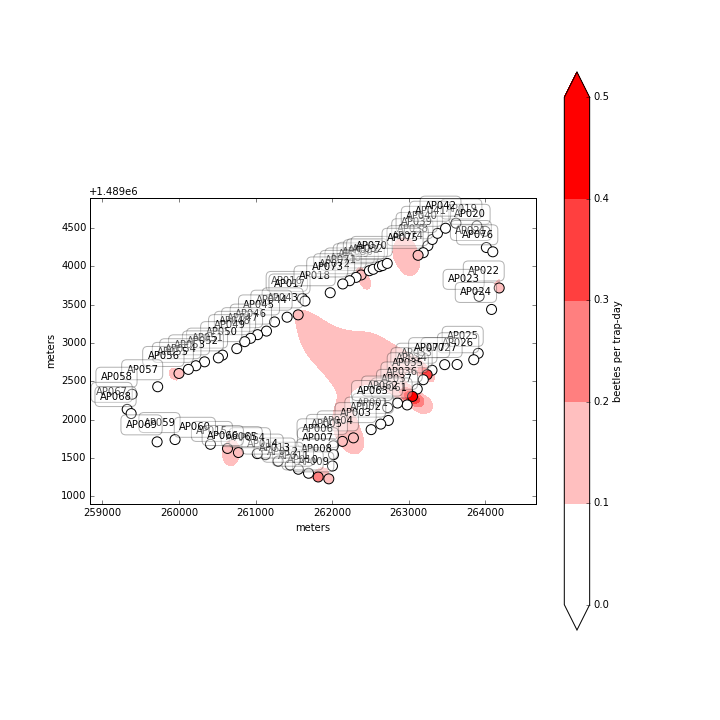
\includegraphics[width=0.6\linewidth,valign=c]{2016-04-01.png}
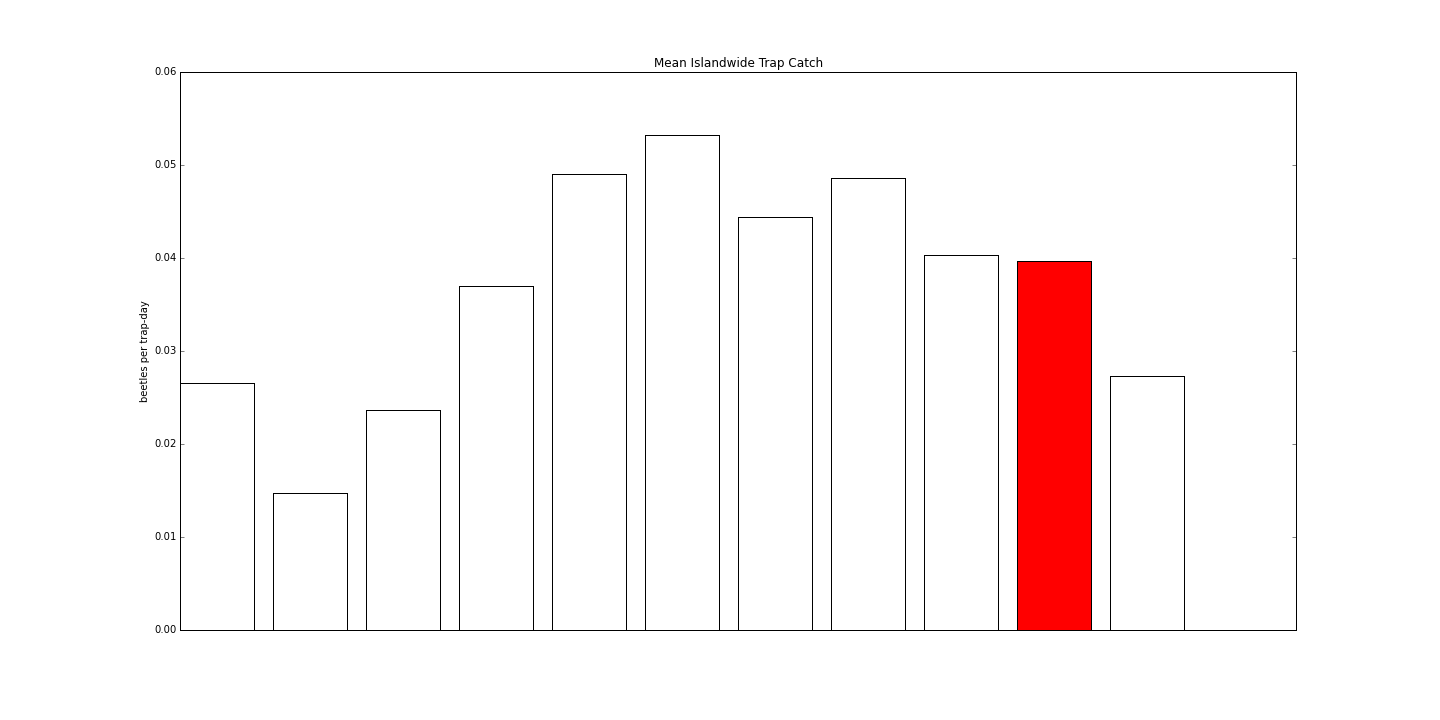
\includegraphics[width=0.4\linewidth,valign=c]{bars2016-04-01.png}
\end{frame}
\begin{frame}{Mean beetles per trap-day for 90 day period ending\\ \textbf{01 May 2016}}
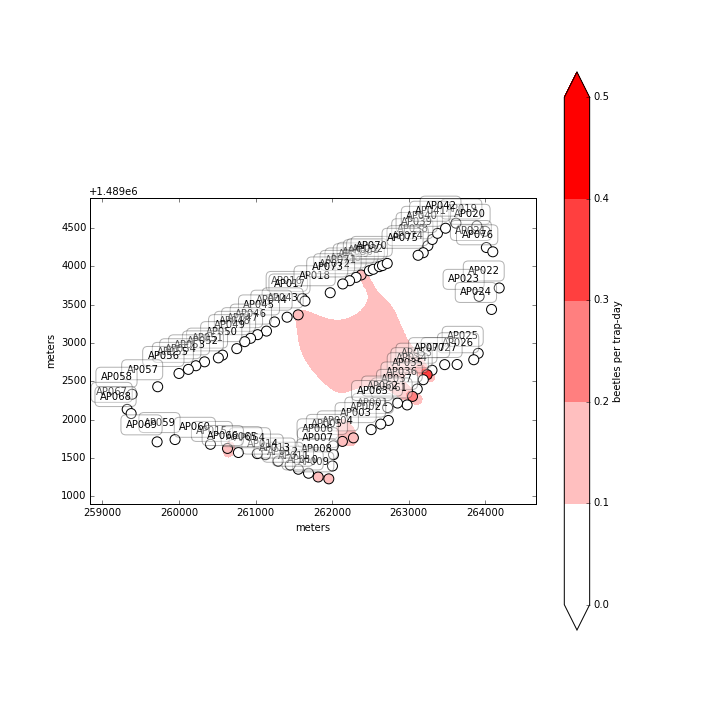
\includegraphics[width=0.6\linewidth,valign=c]{2016-05-01.png}
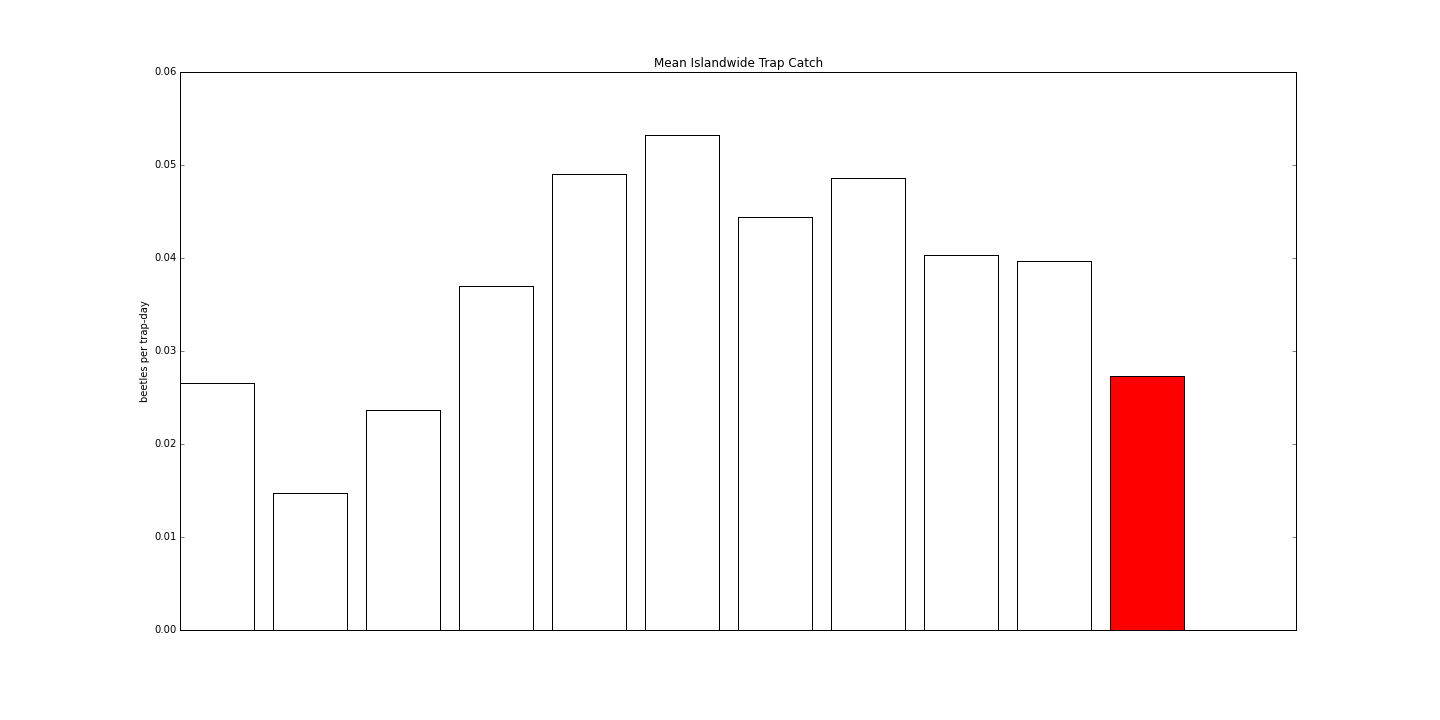
\includegraphics[width=0.4\linewidth,valign=c]{bars2016-05-01.png}
\end{frame}
\end{document}